\label{fnt1.1.1-1}
\subsubsection*{Scientists don't come up with ``right answers.''}

Usually, when your instructor asks you to ``do problems'' for homework or on a test, they expect you to get a ``right answer,'' right? Well, we don't. As a matter of fact, for many of the problems you will encounter in this course, there won't be one ``right answer.'' Science just doesn't work that way. For every problem, there are a number of ways one can approach the problem, and each different solution path might result in different answers. But, that doesn't mean that one of them is ``right'' and the others are not.

\subsubsection*{Scientists come up with arguments.}

Much more important than an answer to a question or problem in science is usually the method by which one arrived at this answer. So, our emphasis is on the method you use to solve a problem -- the pathway to your solution. \textbf{We want to know what assumptions and decisions you're making as you solve a problem, and how you're using these assumptions and decisions to \emph{make an argument} for \emph{your} solution.} That's how science works! There is nobody who knows ``the right answer.'' But there are people who can look at what you've done and tell you whether the assumptions you've made are appropriate in a particular situation and if the argument you've constructed is valid and convincing. In science, this is called ``peer-review'' because the people who look at your work are other scientists.

\subsubsection*{So, if we don't care so much about you ``getting the right answer,'' how will we evaluate your progress in this course?}

Just like in a scientific publication, \textbf{we ask you to be \emph{very specific} about what you did and did not do, and \emph{how} you arrived at a particular solution to a problem.} We'll practice this a lot, so that you know what we expect from you. This first problem is an extreme example of what problem-solving in this class looks like for you: \emph{We'll actually give you some answers.} A little further down, you'll find a box with some answers that one might reasonably get when solving this problem. Note that we're not saying these are the exact answers you will get or that we expect you to get! But your solutions to this problem might be quite similar to the ones given below.

\subsubsection*{Now, if we give you the answers, what do we want you to do?}

We want you to describe in detail how you are using the diagram below to respond to the prompts in the problem. Write a story about the diagram and about how you are reading the graph to get the values you get. While this is stated a few times below, it's worth repeating: \emph{We don't want you to do any calculations for this problem!} Instead, use the diagram and tell us \emph{how} you're using the diagram and \emph{why} we should believe you that your answer to the problem is a reasonable one.

Yes, this might be a bit more work than what you're used to from other classes. Later in this course, we'll find shorter ways for you to show us your work and argument. But for now, \textbf{\emph{please do write out a detailed story -- including your assumptions, decisions, etc. -- for each part of the problem.}}

\subsubsection*{On to the actual problem:}

Use the particular \TempGraph{} of the \ThreePhaseModel{} shown below to respond to the prompts in this FNT.\\

\noindent
{\centering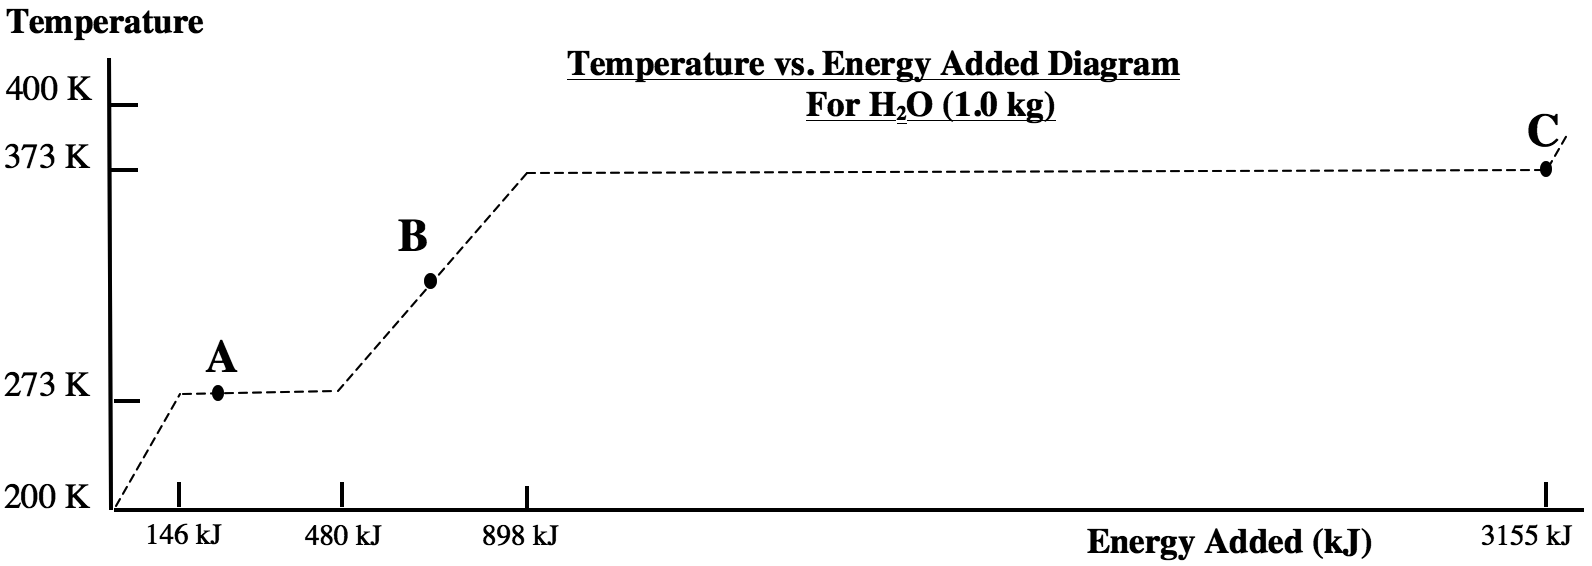
\includegraphics[width=.95\linewidth]{fnt111-1.png}\par}

\noindent The values along the $x$-axis (\unit[146]{kJ}, \unit[480]{kJ}, etc.) are the amounts of energy that must be added to get the \unit[1.0]{kg} of water from an initial temperature of \unit[200]{K} to the next phase change. For example, \unit[480]{kJ} is the total amount of energy that must be added to the water starting at the initial temperature of \unit[200]{K} to completely melt all the ice.

\begin{enumerate}[(a)]
	\item Describe what is happening at each of the ``corners'' on the graph. What phase is the water in at the letter A, B, C?
	\label{fnt1.1.1-1A}
	
	\item Assume that you have one kilogram of water at an initial temperature of \unit[200]{K}. If \unit[795]{kJ} of energy is added, describe the final state (approximate temperature and phase) of the water. If the water is in a mixed phase, determine very approximately the percent in each phase.
	
		You are not expected to do any calculations at this time. Simply tell us what the diagram tells you (and how you know that it does).
	\label{fnt1.1.1-1B}
	
	\item Repeat \hyperref[fnt1.1.1-1B]{Part~\ref*{fnt1.1.1-1B}} but with \unit[146]{kJ} of energy added to the water initially at \unit[200]{K}.
	
	\item Repeat \hyperref[fnt1.1.1-1B]{Part~\ref*{fnt1.1.1-1B}} but with \unit[1650]{kJ} of energy added to the water initially at \unit[200]{K}.
	
	\item State the initial and final conditions of the process that takes the system from Point C to Point B and determine very approximately how much energy would have to be added or removed.
	\label{fnt1.1.1-1C}
	
	\item Repeat \hyperref[fnt1.1.1-1C]{Part~\ref*{fnt1.1.1-1C}} for water initially in State A and ending in State C.
	\label{fnt1.1.1-1D}
	
\end{enumerate}

\subsubsection*{Again: Do not make any calculations to respond to these prompts!}